\documentclass[]{article}
\usepackage{lmodern}
\usepackage{amssymb,amsmath}
\usepackage{ifxetex,ifluatex}
\usepackage{fixltx2e} % provides \textsubscript
\ifnum 0\ifxetex 1\fi\ifluatex 1\fi=0 % if pdftex
  \usepackage[T1]{fontenc}
  \usepackage[utf8]{inputenc}
\else % if luatex or xelatex
  \ifxetex
    \usepackage{mathspec}
    \usepackage{xltxtra,xunicode}
  \else
    \usepackage{fontspec}
  \fi
  \defaultfontfeatures{Mapping=tex-text,Scale=MatchLowercase}
  \newcommand{\euro}{€}
\fi
% use upquote if available, for straight quotes in verbatim environments
\IfFileExists{upquote.sty}{\usepackage{upquote}}{}
% use microtype if available
\IfFileExists{microtype.sty}{%
\usepackage{microtype}
\UseMicrotypeSet[protrusion]{basicmath} % disable protrusion for tt fonts
}{}
\usepackage[margin=1in]{geometry}
\usepackage{longtable,booktabs}
\usepackage{graphicx}
\usepackage{subfigure}
\makeatletter
\def\maxwidth{\ifdim\Gin@nat@width>\linewidth\linewidth\else\Gin@nat@width\fi}
\def\maxheight{\ifdim\Gin@nat@height>\textheight\textheight\else\Gin@nat@height\fi}
\makeatother
% Scale images if necessary, so that they will not overflow the page
% margins by default, and it is still possible to overwrite the defaults
% using explicit options in \includegraphics[width, height, ...]{}
\setkeys{Gin}{width=\maxwidth,height=\maxheight,keepaspectratio}
\ifxetex
  \usepackage[setpagesize=false, % page size defined by xetex
              unicode=false, % unicode breaks when used with xetex
              xetex]{hyperref}
\else
  \usepackage[unicode=true]{hyperref}
\fi
\hypersetup{breaklinks=true,
            bookmarks=true,
            pdfauthor={},
            pdftitle={4\^{}\{th\} Report},
            colorlinks=true,
            citecolor=blue,
            urlcolor=blue,
            linkcolor=magenta,
            pdfborder={0 0 0}}
\urlstyle{same}  % don't use monospace font for urls
\setlength{\parindent}{0pt}
\setlength{\parskip}{6pt plus 2pt minus 1pt}
\setlength{\emergencystretch}{3em}  % prevent overfull lines
\setcounter{secnumdepth}{5}

%%% Use protect on footnotes to avoid problems with footnotes in titles
\let\rmarkdownfootnote\footnote%
\def\footnote{\protect\rmarkdownfootnote}

%%% Change title format to be more compact
\usepackage{titling}

% Create subtitle command for use in maketitle
\newcommand{\subtitle}[1]{
  \posttitle{
    \begin{center}\large#1\end{center}
    }
}

\setlength{\droptitle}{-2em}
  \title{Report}
  \pretitle{\vspace{\droptitle}\centering\huge}
  \posttitle{\par}
  \author{}
  \preauthor{}\postauthor{}
  \predate{\centering\large\emph}
  \postdate{\par}
  %\date{7th of July}



\begin{document}

\maketitle


%\section{Mothedology}


%% Date and time: ma, jul 11, 2016 - 17:00:47
%\begin{table}[!htbp] \centering 
%  \caption{} 
%  \label{} 
%\begin{tabular}{@{\extracolsep{5pt}}lccccc} 
%\\[-1.8ex]\hline 
%\hline \\[-1.8ex] 
%Statistic & \multicolumn{1}{c}{N} & \multicolumn{1}{c}{Mean} & \multicolumn{1}{c}{St. Dev.} & \multicolumn{1}{c}{Min} & \multicolumn{1}{c}{Max} \\ 
%\hline \\[-1.8ex] 
%X1 & 1,000 & 1.299 & 0.235 & 0.351 & 2.159 \\ 
%X2 & 1,000 & 0.026 & 0.007 & $-$0.043 & 0.051 \\ 
%X3 & 1,000 & 0.191 & 0.035 & 0.081 & 0.329 \\ 
%V4 & 1,000 & 42.252 & 25.180 & $-$255.697 & 644.446 \\ 
%\hline \\[-1.8ex] 
%\end{tabular} 
%\end{table} 
%% Table created by stargazer v.5.2 by Marek Hlavac, Harvard University. E-mail: hlavac at fas.harvard.edu
%% Date and time: ma, jul 11, 2016 - 11:10:49



%%%%%%%%%%%%  aca voy..


\begin{table}[!htbp] \centering 
  \caption{Estimations of 1000 simulations, with $\lambda_0=0.8$, $\beta_0=0.0175$ and $\mu_0=0.1$. The initial parameter was $(800,18,100)$.} 
  \label{} 
\begin{tabular}{@{\extracolsep{5pt}}lccccc} 
\\[-1.8ex]\hline 
\hline \\[-1.8ex] 
Statistic &  \multicolumn{1}{c}{Mean} & \multicolumn{1}{c}{St. Dev.} & \multicolumn{1}{c}{Min} & \multicolumn{1}{c}{Max} \\ 
\hline \\[-1.8ex] 
$\lambda_0$  & 1.299 & 0.235 & 0.351 & 2.159  \\ 
$\beta_0$  & 0.026 & 0.007 & $-$0.043 & 0.051 \\ 
$\mu_0$ &  & 0.191 & 0.035 & 0.081 & 0.329 \\ 
%$K$ &  31.027 & 355.579 & $-$11,177.170 & 644.446 \\ 
\hline \\[-1.8ex] 
\end{tabular} 
\end{table}
 \begin{figure}[h]
\centering
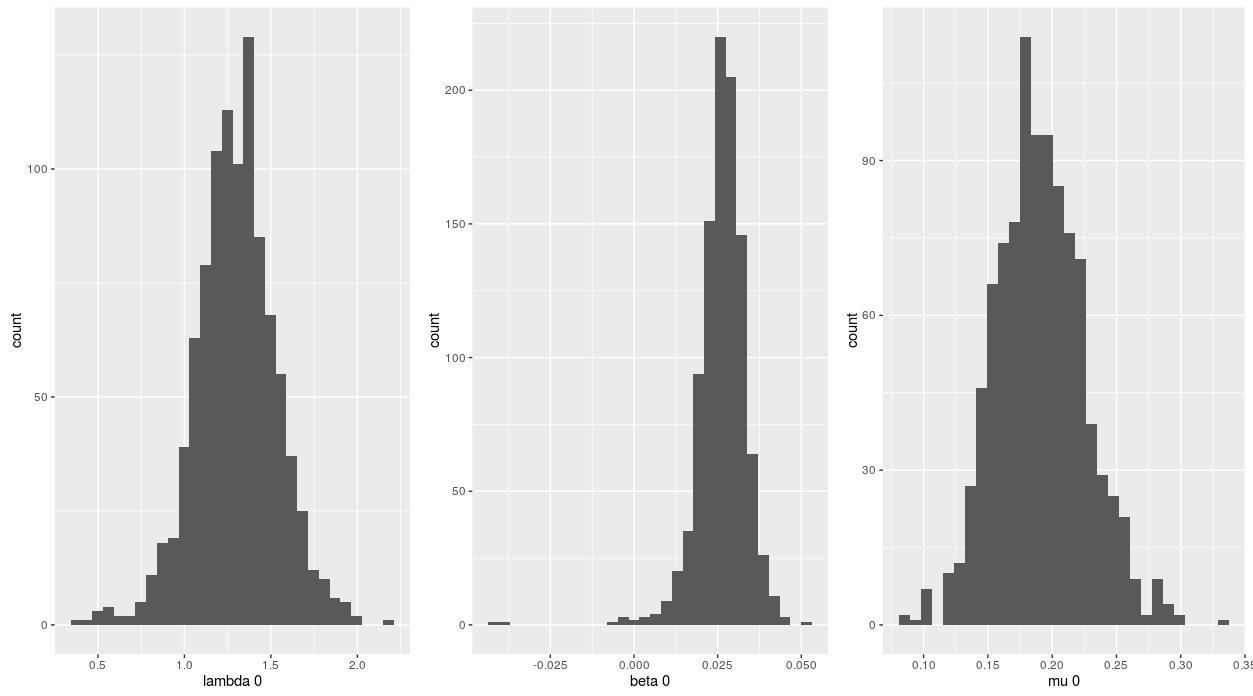
\includegraphics[width=.8\textwidth]{mu01.png}
\end{figure}

%\begin{figure}[t]
%\centering
%\subfigure[text]{
%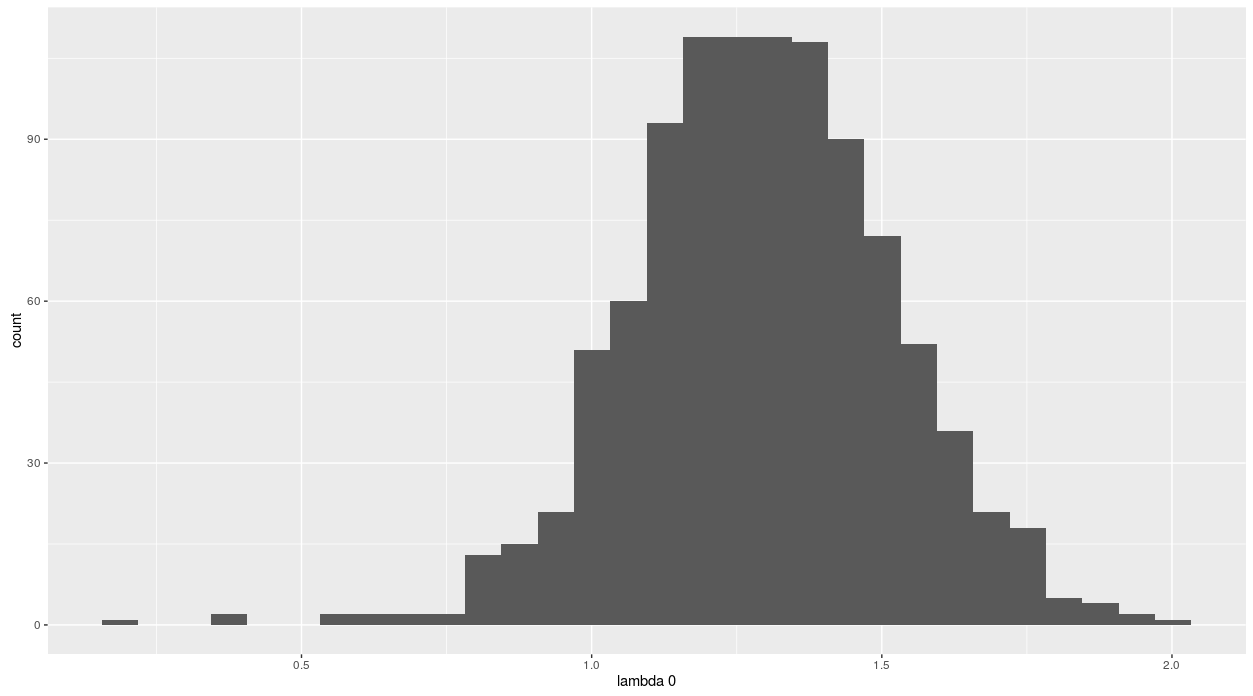
\includegraphics[width=.525\textwidth]{lambda0.png}
%}
%\subfigure[text]{
%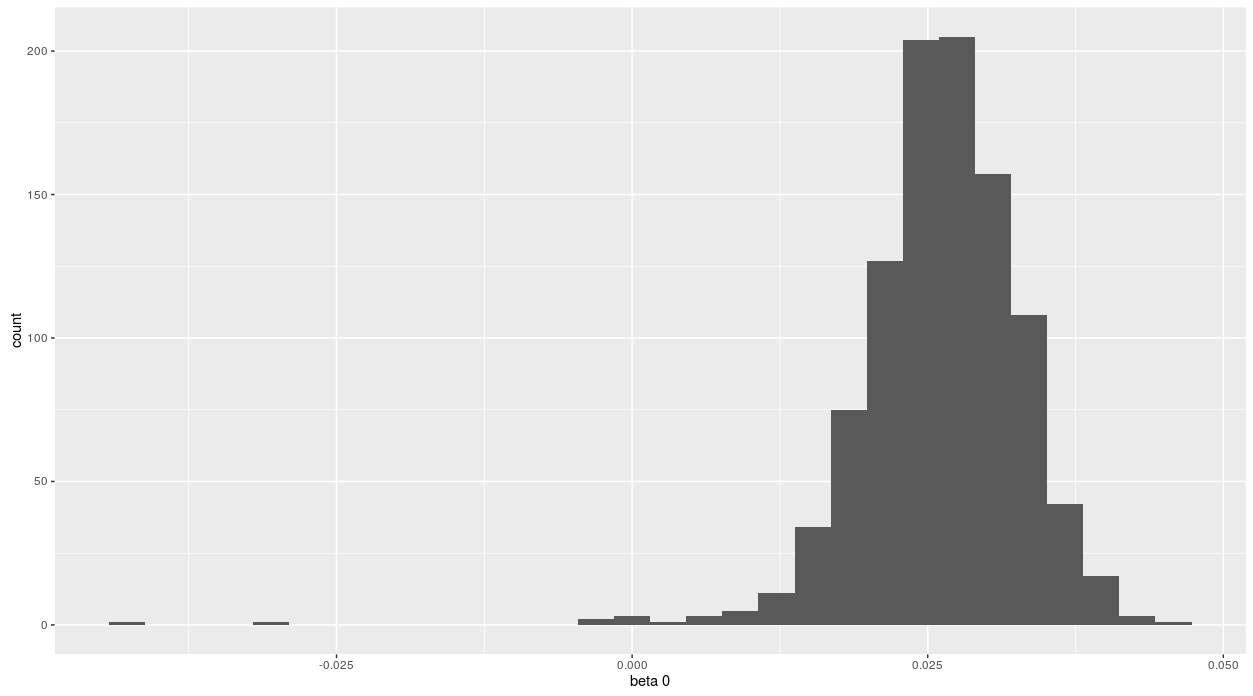
\includegraphics[width=.525\textwidth]{beta0.png}
%}
%
%\subfigure[text]{
%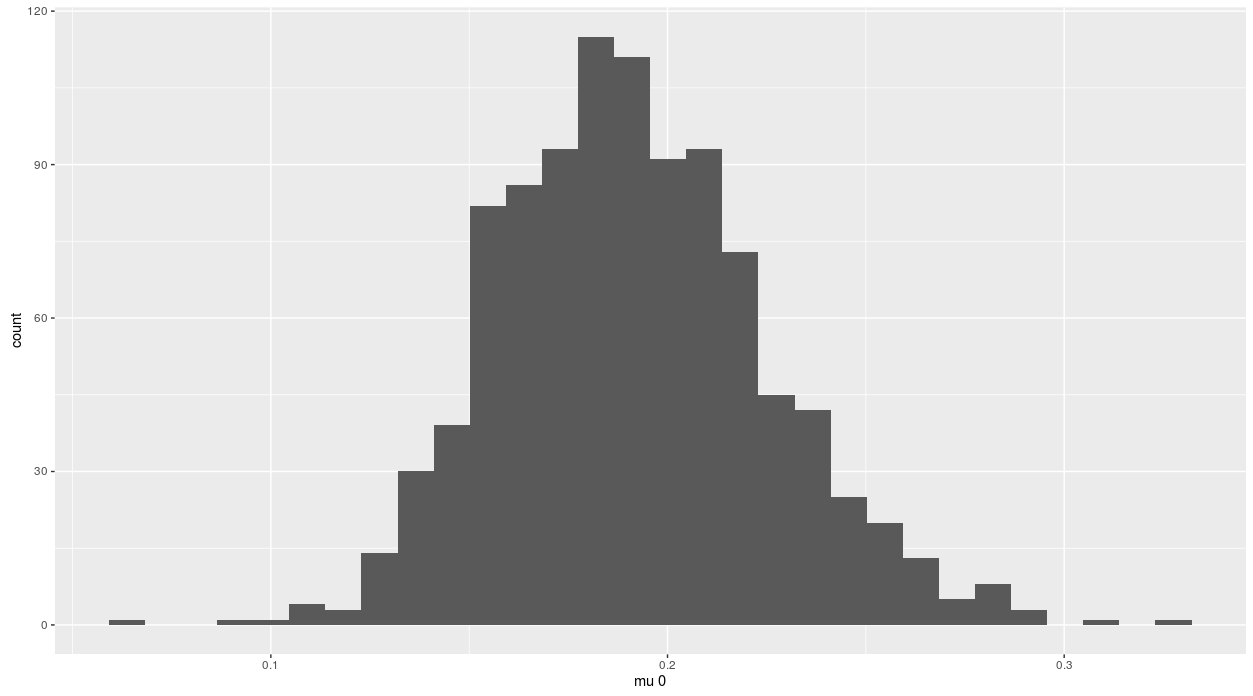
\includegraphics[width=.525\textwidth]{mu0.png}
%}
%
%\end{figure}
%
%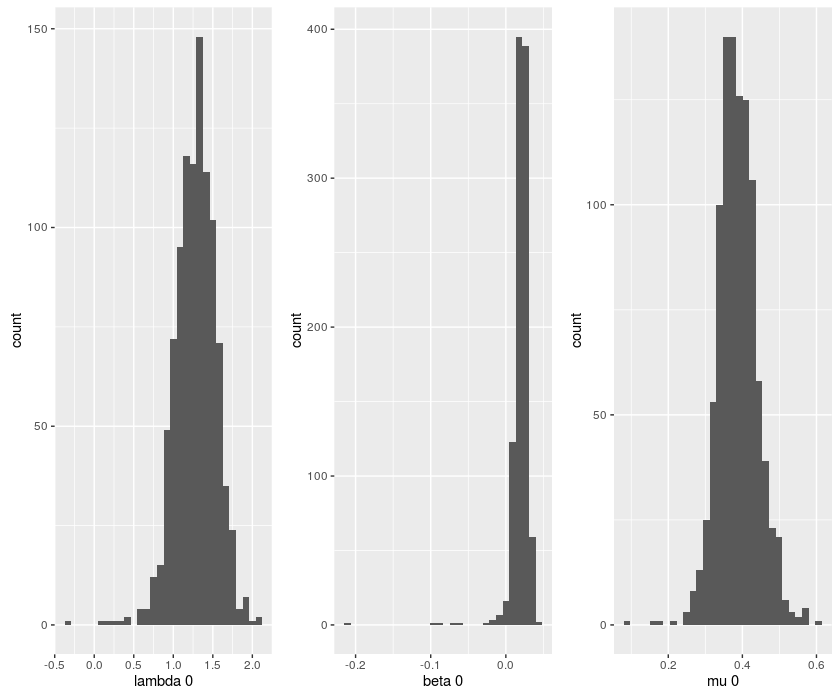
\includegraphics[width=.8\textwidth]{mu02.png}
%

% Table created by stargazer v.5.2 by Marek Hlavac, Harvard University. E-mail: hlavac at fas.harvard.edu
% Date and time: ma, jul 11, 2016 - 13:44:27
\newpage
\begin{table}[!htbp] \centering 
  \caption{} 
  \label{} 
\begin{tabular}{@{\extracolsep{5pt}}lccccc} 
\\[-1.8ex]\hline 
\hline \\[-1.8ex] 
Statistic & \multicolumn{1}{c}{N} & \multicolumn{1}{c}{Mean} & \multicolumn{1}{c}{St. Dev.} & \multicolumn{1}{c}{Min} & \multicolumn{1}{c}{Max} \\ 
\hline \\[-1.8ex] 
X1 & 1,000 & 1.284 & 0.326 & $-$0.288 & 2.059 \\ 
X2 & 1,000 & 0.004 & 0.035 & $-$0.439 & 0.089 \\ 
X3 & 1,000 & 0.772 & 0.089 & 0.464 & 1.167 \\ 
V4 & 1,000 & 33.833 & 1,327.034 & $-$36,730.000 & 16,236.080 \\ 
\hline \\[-1.8ex] 
\end{tabular} 
\end{table} 
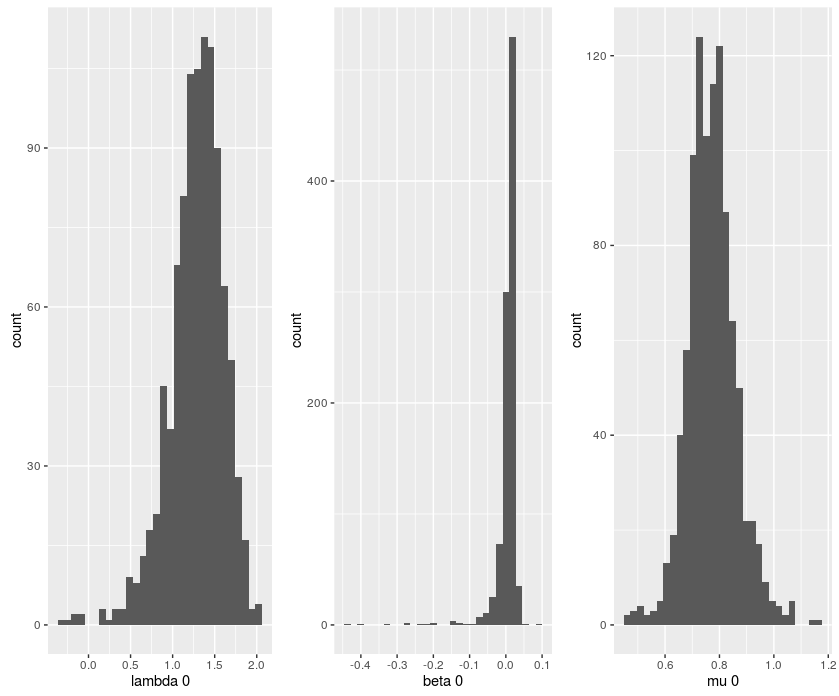
\includegraphics[width=.8\textwidth]{mu04.png}

% latex table generated in R 3.2.1 by xtable 1.8-0 package \% Fri Jan
\newpage


% Date and time: di, jul 12, 2016 - 10:34:35
\begin{table}[!htbp] \centering 
  \caption{} 
  \label{} 
\begin{tabular}{@{\extracolsep{5pt}}lccccc} 
\\[-1.8ex]\hline 
\hline \\[-1.8ex] 
Statistic & \multicolumn{1}{c}{N} & \multicolumn{1}{c}{Mean} & \multicolumn{1}{c}{St. Dev.} & \multicolumn{1}{c}{Min} & \multicolumn{1}{c}{Max} \\ 
\hline \\[-1.8ex] 
X1 & 1,000 & 1.291 & 0.340 & $-$0.292 & 2.274 \\ 
X2 & 1,000 & 0.004 & 0.033 & $-$0.326 & 0.069 \\ 
X3 & 1,000 & 0.770 & 0.092 & 0.333 & 1.167 \\ 
V4 & 1,000 & 50.721 & 6,691.263 & $-$92,207.600 & 179,176.300 \\ 
\hline \\[-1.8ex] 
\end{tabular} 
\end{table} 


\newpage

% Table created by stargazer v.5.2 by Marek Hlavac, Harvard University. E-mail: hlavac at fas.harvard.edu
% Date and time: di, jul 12, 2016 - 11:14:20
\begin{table}[!htbp] \centering 
  \caption{} 
  \label{} 
\begin{tabular}{@{\extracolsep{5pt}}lccccc} 
\\[-1.8ex]\hline 
\hline \\[-1.8ex] 
Statistic & \multicolumn{1}{c}{N} & \multicolumn{1}{c}{Mean} & \multicolumn{1}{c}{St. Dev.} & \multicolumn{1}{c}{Min} & \multicolumn{1}{c}{Max} \\ 
\hline \\[-1.8ex] 
X1 & 1,000 & 0.841 & 0.060 & $-$0.035 & 1.061 \\ 
X2 & 1,000 & 0.018 & 0.011 & $-$0.242 & 0.024 \\ 
X3 & 1,000 & 0.109 & 0.018 & 0.050 & 0.324 \\ 
V4 & 1,000 & 39.619 & 3.652 & $-$43.967 & 67.607 \\ 
\hline \\[-1.8ex] 
\end{tabular} 
\end{table} 


% Date and time: di, jul 12, 2016 - 11:56:27
\begin{table}[!htbp] \centering 
  \caption{} 
  \label{} 
\begin{tabular}{@{\extracolsep{5pt}}lccccc} 
\\[-1.8ex]\hline 
\hline \\[-1.8ex] 
Statistic & \multicolumn{1}{c}{N} & \multicolumn{1}{c}{Mean} & \multicolumn{1}{c}{St. Dev.} & \multicolumn{1}{c}{Min} & \multicolumn{1}{c}{Max} \\ 
\hline \\[-1.8ex] 
X1 & 1,000 & 0.843 & 0.060 & 0.116 & 1.132 \\ 
X2 & 1,000 & 0.018 & 0.004 & $-$0.101 & 0.025 \\ 
X3 & 1,000 & 0.109 & 0.018 & 0.063 & 0.305 \\ 
V4 & 1,000 & 39.244 & 12.885 & $-$346.914 & 44.562 \\ 
\hline \\[-1.8ex] 
\end{tabular} 
\end{table} 

\newpage
\begin{table}[!htbp] \centering 
  \caption{} 
  \label{} 
\begin{tabular}{@{\extracolsep{5pt}}lccccc} 
\\[-1.8ex]\hline 
\hline \\[-1.8ex] 
Statistic & \multicolumn{1}{c}{N} & \multicolumn{1}{c}{Mean} & \multicolumn{1}{c}{St. Dev.} & \multicolumn{1}{c}{Min} & \multicolumn{1}{c}{Max} \\ 
\hline \\[-1.8ex] 
X1 & 1,000 & 1.587 & 0.638 & 0.253 & 7.048 \\ 
X2 & 1,000 & 0.034 & 0.016 & $-$0.076 & 0.157 \\ 
X3 & 1,000 & 0.202 & 0.056 & 0.070 & 0.776 \\ 
%V4 & 1,000 & 40.393 & 7.930 & $-$50.310 & 222.981 \\ 
\hline \\[-1.8ex] 
\end{tabular} 
\end{table} 

 \begin{figure}[h]
\centering
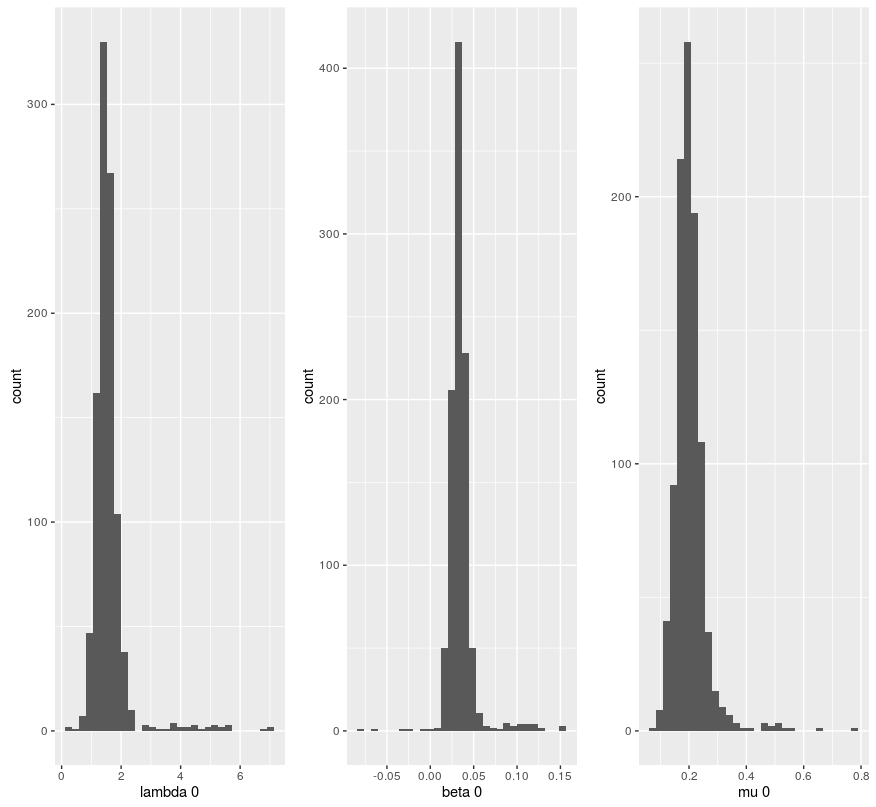
\includegraphics[width=.5\textwidth]{mu01v3.png}
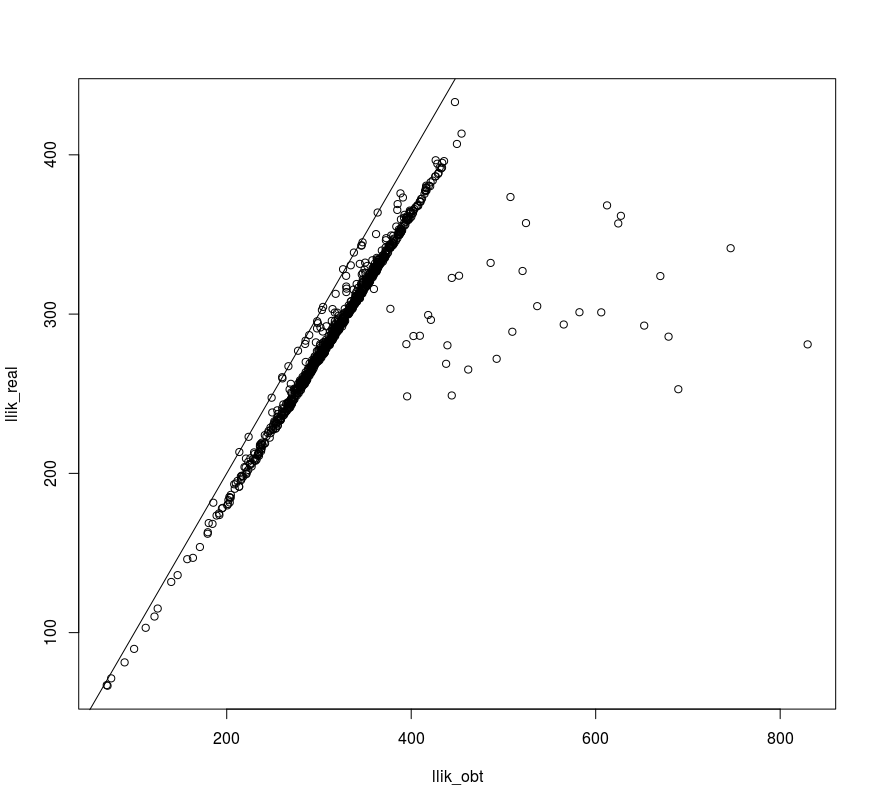
\includegraphics[width=.5\textwidth]{llikv3.png}
\end{figure}


\begin{table}[!htbp] \centering 
  \caption{} 
  \label{} 
\begin{tabular}{@{\extracolsep{5pt}}lccccc} 
\\[-1.8ex]\hline 
\hline \\[-1.8ex] 
Statistic & \multicolumn{1}{c}{N} & \multicolumn{1}{c}{Mean} & \multicolumn{1}{c}{St. Dev.} & \multicolumn{1}{c}{Min} & \multicolumn{1}{c}{Max} \\ 
\hline \\[-1.8ex] 
X1 & 1,000 & 1.560 & 0.311 & 0.597 & 2.702 \\ 
X2 & 1,000 & 0.034 & 0.008 & $-$0.017 & 0.064 \\ 
X3 & 1,000 & 0.197 & 0.037 & 0.084 & 0.479 \\ 
%V4 & 1,000 & 39.479 & 17.189 & $-$393.966 & 64.283 \\ 
\hline \\[-1.8ex] 
\end{tabular} 
\end{table} 

 \begin{figure}[h]
\centering
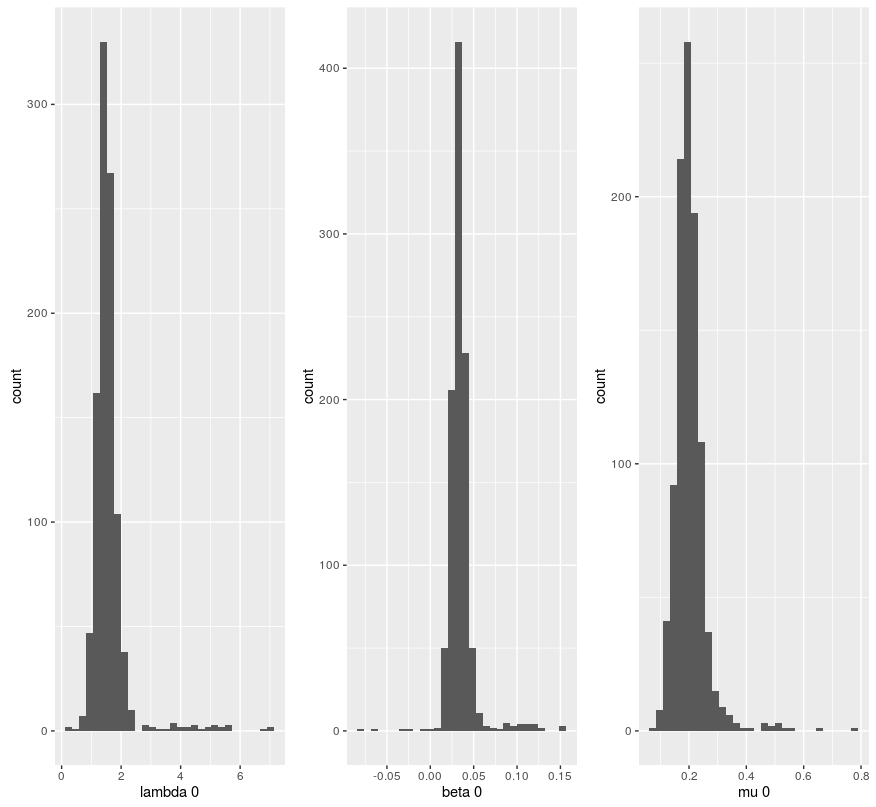
\includegraphics[width=.5\textwidth]{mu01v3.png}
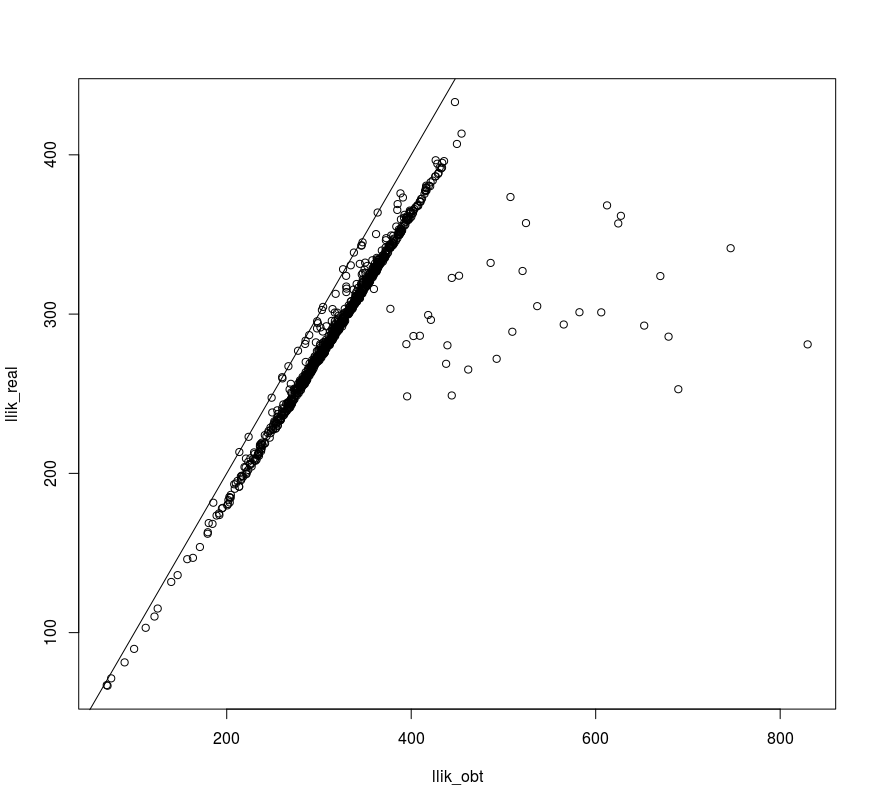
\includegraphics[width=.5\textwidth]{llikv3.png}
\end{figure}

\newpage

with real initial parameters 



 \begin{figure}[h]
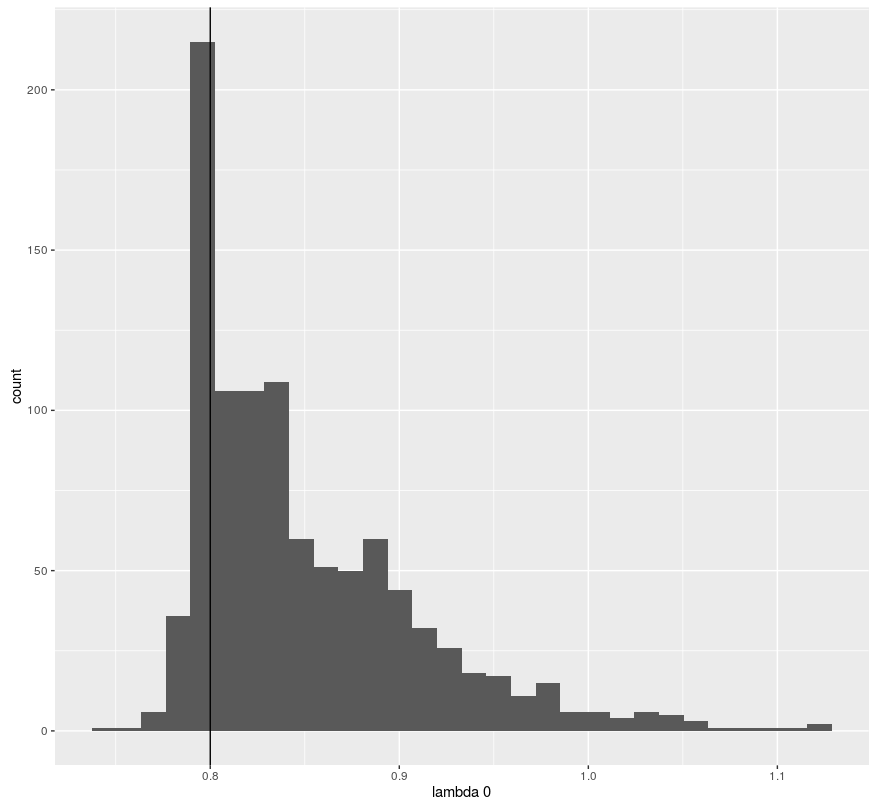
\includegraphics[width=.5\textwidth]{lambdar.png}
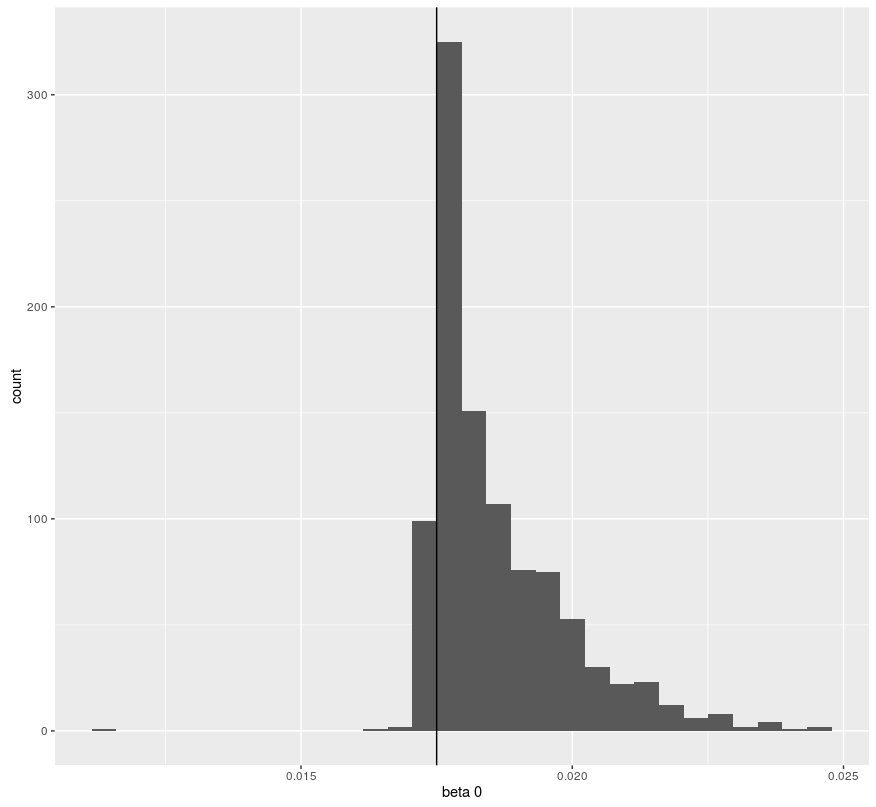
\includegraphics[width=.5\textwidth]{beta0r.png}
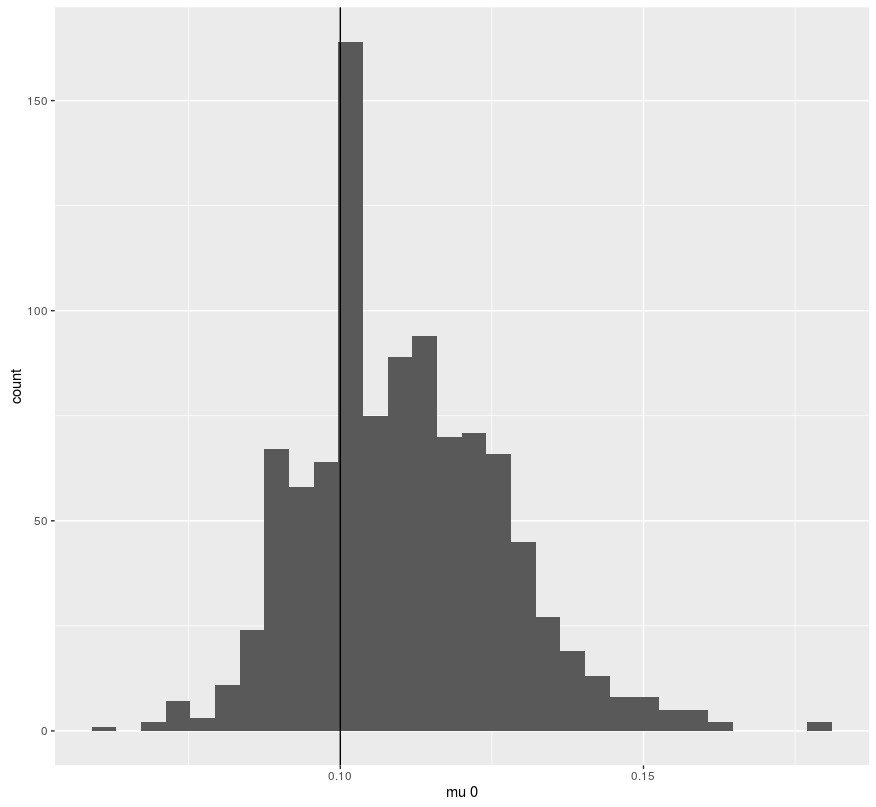
\includegraphics[width=.5\textwidth]{mur.png}
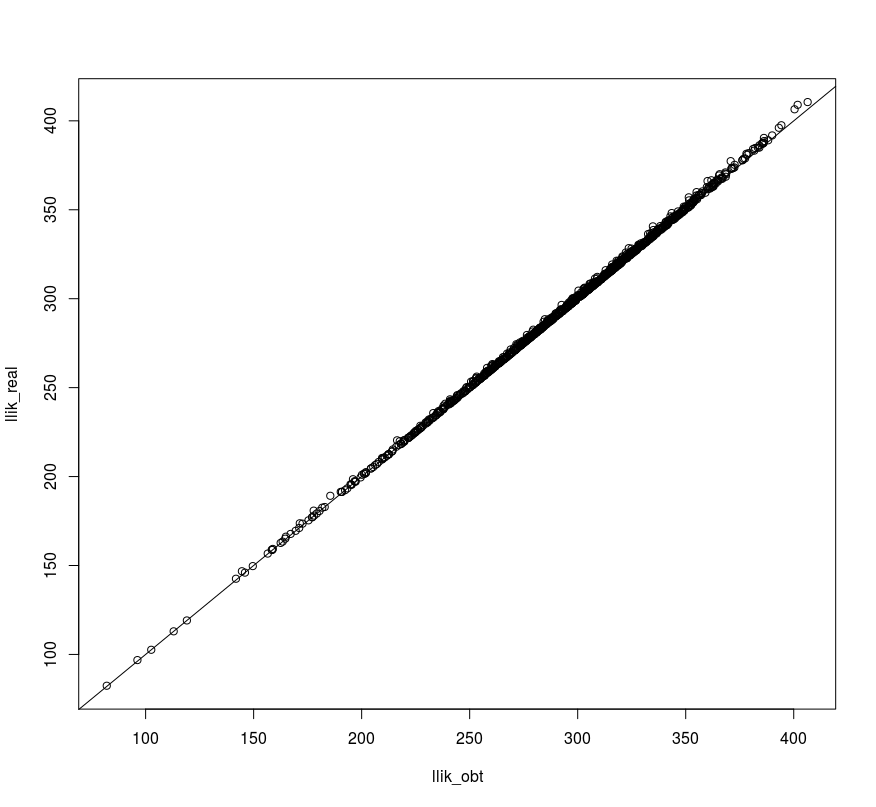
\includegraphics[width=.5\textwidth]{llikr.png}
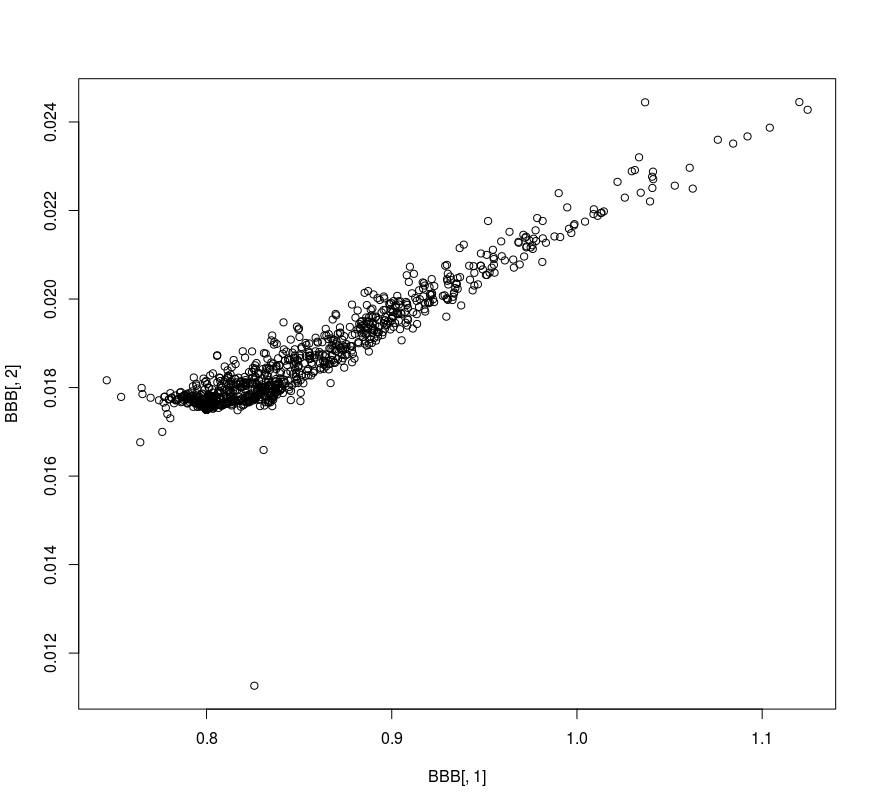
\includegraphics[width=.5\textwidth]{b0lr.png}
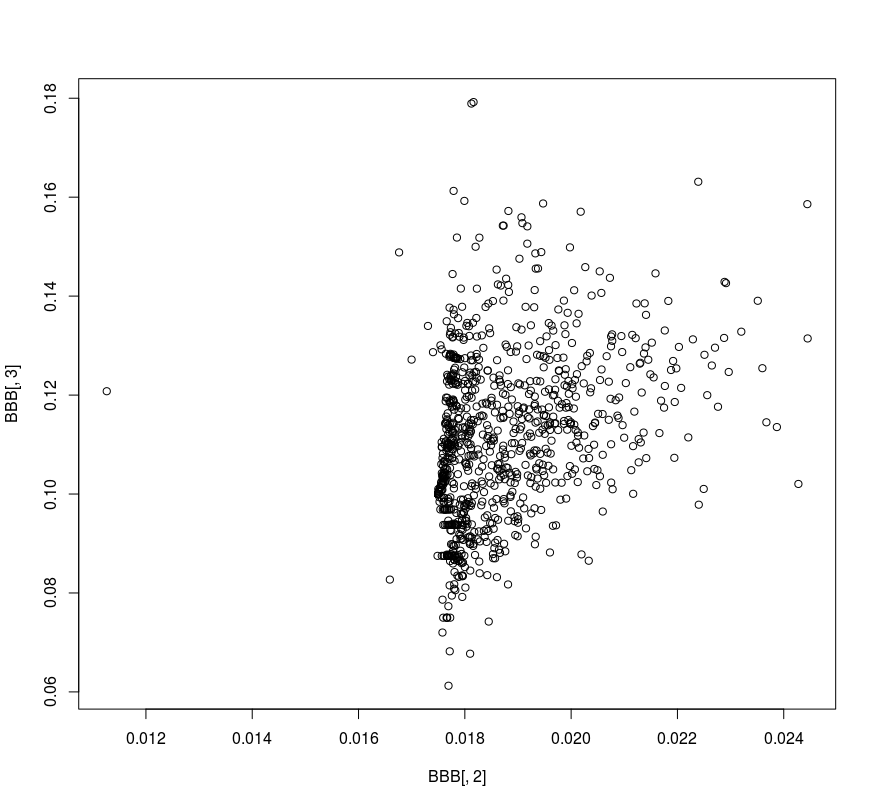
\includegraphics[width=.5\textwidth]{b0mr.png}

\end{figure}

\begin{table}[!htbp] \centering 
  \caption{initial true values} 
  \label{} 
\begin{tabular}{@{\extracolsep{5pt}}lccccc} 
\\[-1.8ex]\hline 
\hline \\[-1.8ex] 
Statistic & \multicolumn{1}{c}{real values} & \multicolumn{1}{c}{Mean} & \multicolumn{1}{c}{St. Dev.} & \multicolumn{1}{c}{Min} & \multicolumn{1}{c}{Max} \\ 
\hline \\[-1.8ex] 
$\lambda_0$ & 0.8 & 0.850 & 0.060 & 0.746 & 1.125 \\ 
$\beta_0$ & 0.0175 & 0.019 & 0.001 & 0.011 & 0.024 \\ 
$\mu_0$ & 0.1 & 0.110 & 0.016 & 0.061 & 0.179 \\ 
$K$ & 40 & 39.734 & 1.758 & 31.210 & 62.598 \\ 
\hline \\[-1.8ex] 
\end{tabular} 
\end{table} 


\newpage

 \begin{figure}[h]
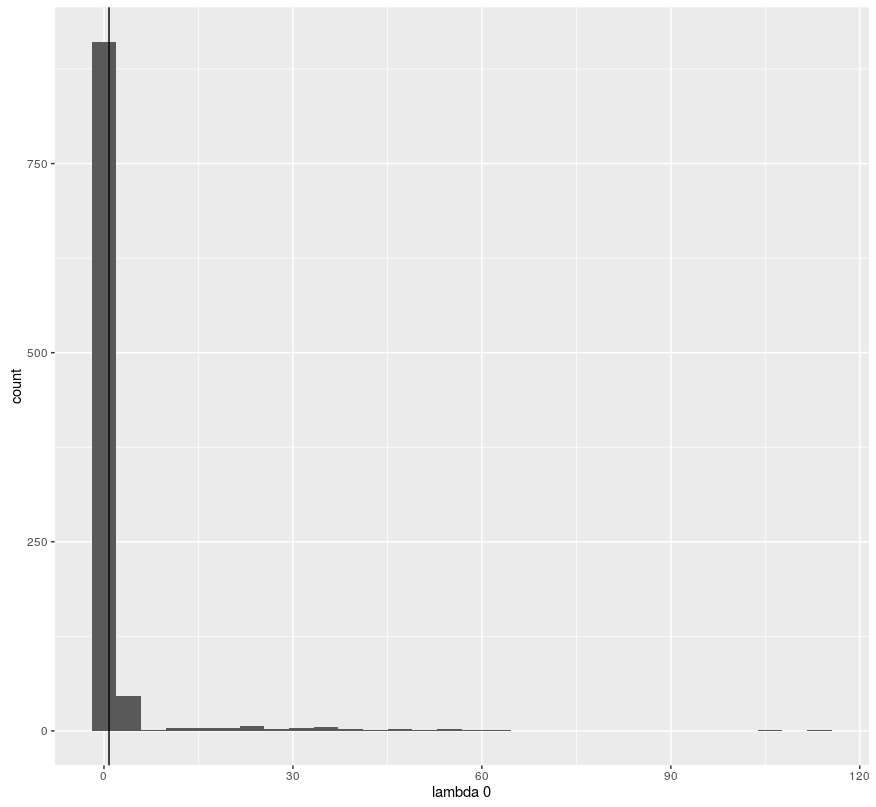
\includegraphics[width=.5\textwidth]{lambdaf.png}
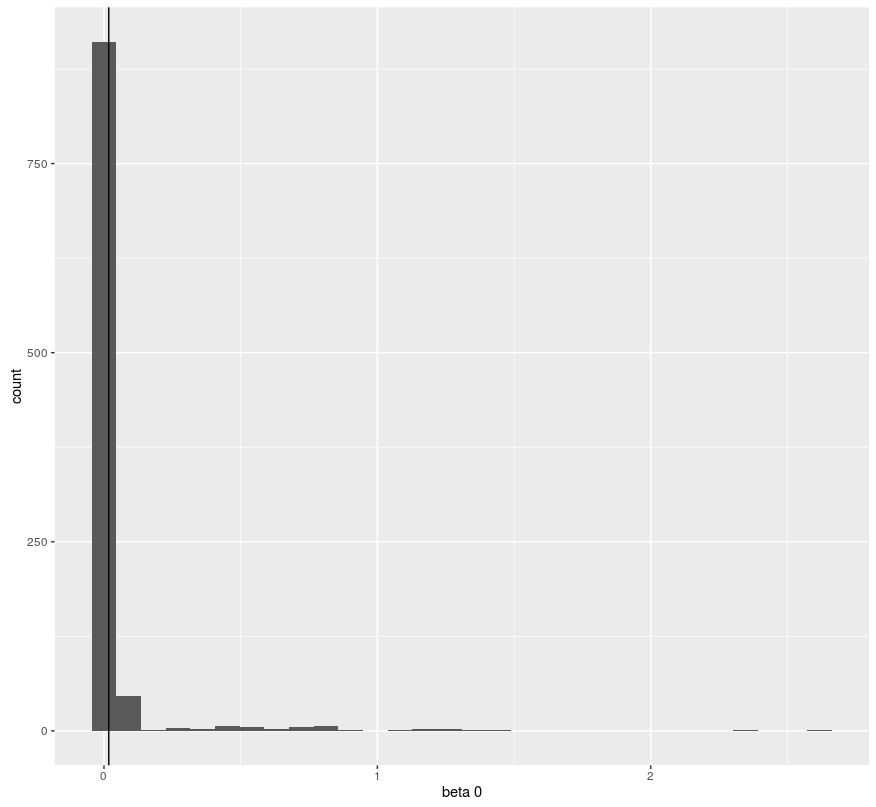
\includegraphics[width=.5\textwidth]{beta0f.png}
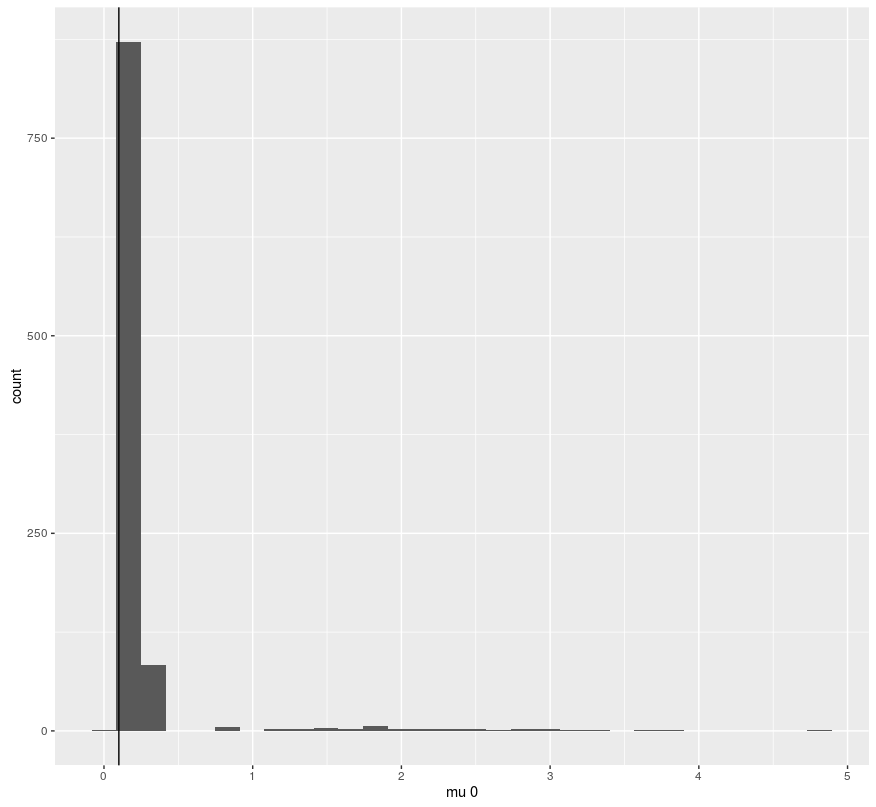
\includegraphics[width=.5\textwidth]{muf.png}
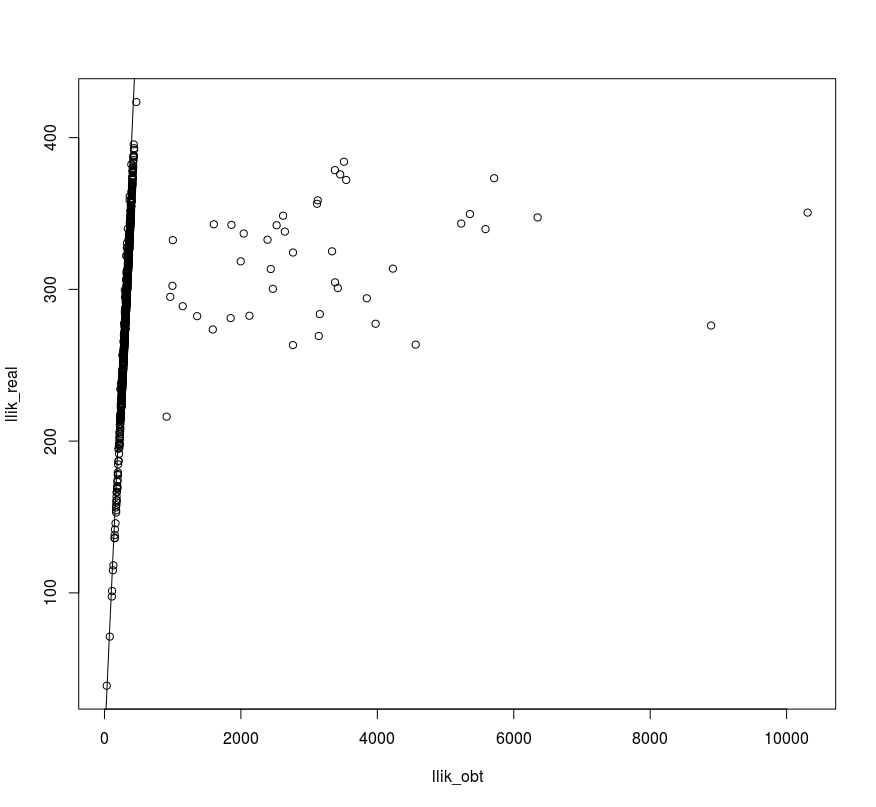
\includegraphics[width=.5\textwidth]{llikf.png}
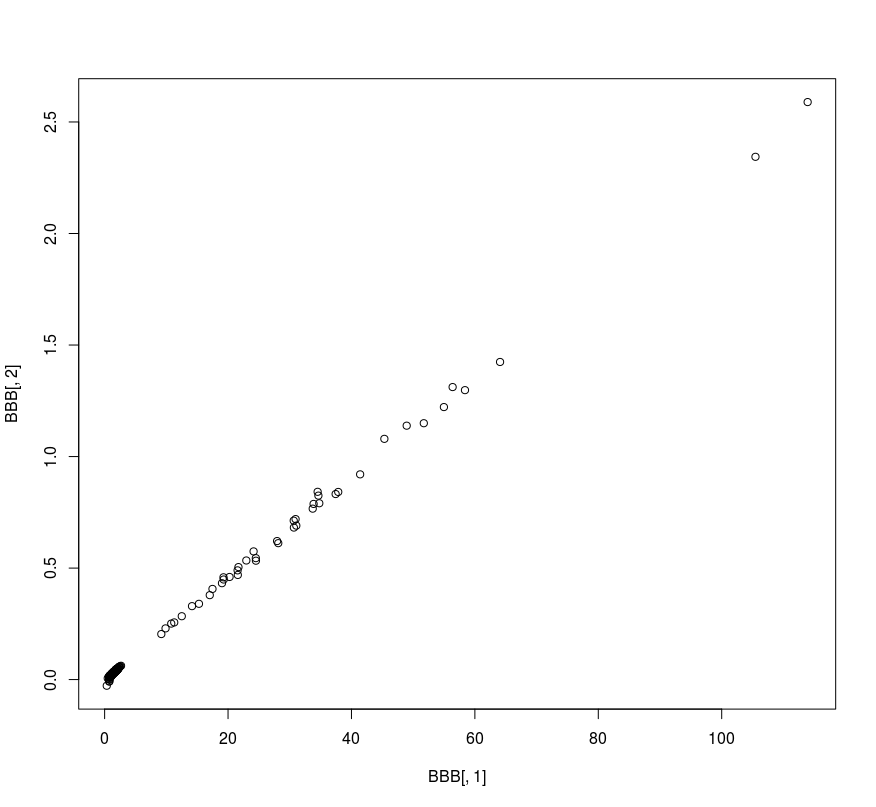
\includegraphics[width=.5\textwidth]{b0lf.png}
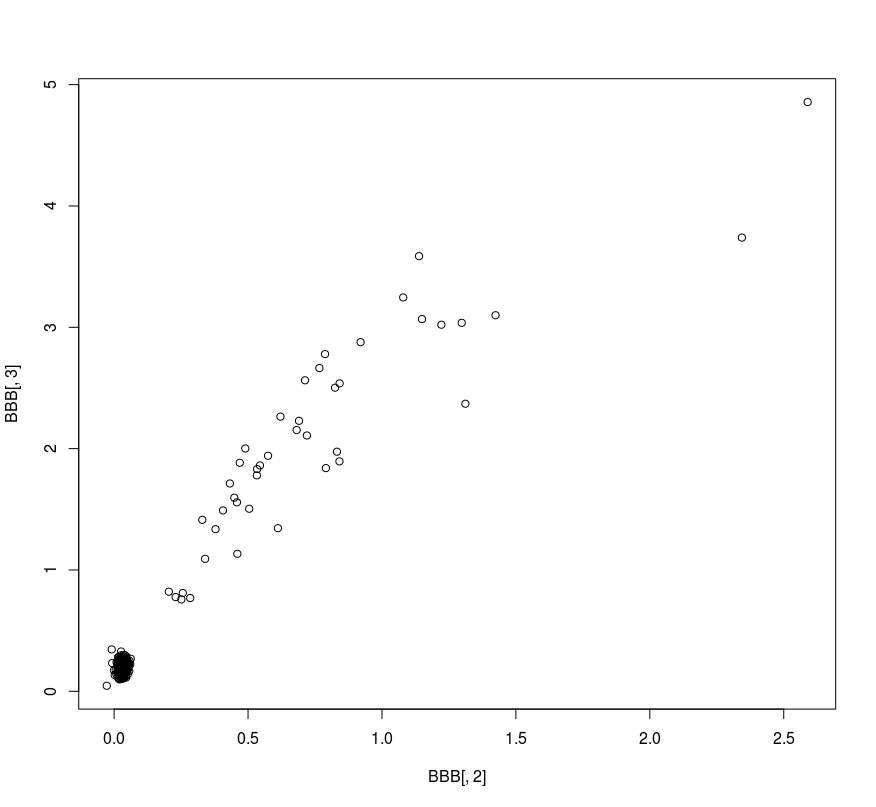
\includegraphics[width=.5\textwidth]{b0mf.png}

\end{figure}



% Date and time: di, jul 12, 2016 - 12:46:40
\begin{table}[!htbp] \centering 
  \caption{starting values (800,10,100)} 
  \label{} 
\begin{tabular}{@{\extracolsep{5pt}}lccccc} 
\\[-1.8ex]\hline 
\hline \\[-1.8ex] 
Statistic & \multicolumn{1}{c}{real value} & \multicolumn{1}{c}{Mean} & \multicolumn{1}{c}{St. Dev.} & \multicolumn{1}{c}{Min} & \multicolumn{1}{c}{Max} \\ 
\hline \\[-1.8ex] 
$\lambda_0$ & 0.8 & 2.850 & 7.858 & 0.345 & 113.927 \\ 
$\beta_0$ & 0.0175 & 0.063 & 0.178 & $-$0.028 & 2.589 \\ 
$\mu_0$ & 0.1 & 0.279 & 0.427 & 0.046 & 4.856 \\ 
$K$ & 40 & 39.562 & 32.295 & $-$937.155 & 276.762 \\ 
\hline \\[-1.8ex] 
\end{tabular} 
\end{table} 

\newpage




% Table created by stargazer v.5.2 by Marek Hlavac, Harvard University. E-mail: hlavac at fas.harvard.edu
% Date and time: di, jul 12, 2016 - 13:25:39
\begin{table}[!htbp] \centering 
  \caption{starting values (0.3,0.005,0.5)} 
  \label{} 
\begin{tabular}{@{\extracolsep{5pt}}lccccc} 
\\[-1.8ex]\hline 
\hline \\[-1.8ex] 
Statistic & \multicolumn{1}{c}{N} & \multicolumn{1}{c}{Mean} & \multicolumn{1}{c}{St. Dev.} & \multicolumn{1}{c}{Min} & \multicolumn{1}{c}{Max} \\ 
\hline \\[-1.8ex] 
X1 & 1,000 & 1.283 & 0.297 & 0.499 & 2.281 \\ 
X2 & 1,000 & 0.026 & 0.009 & $-$0.022 & 0.053 \\ 
X3 & 1,000 & 0.198 & 0.032 & 0.038 & 0.288 \\ 
V4 & 1,000 & 41.957 & 73.794 & $-$1,917.311 & 667.766 \\ 
\hline \\[-1.8ex] 
\end{tabular} 
\end{table} 

 \begin{figure}[h]
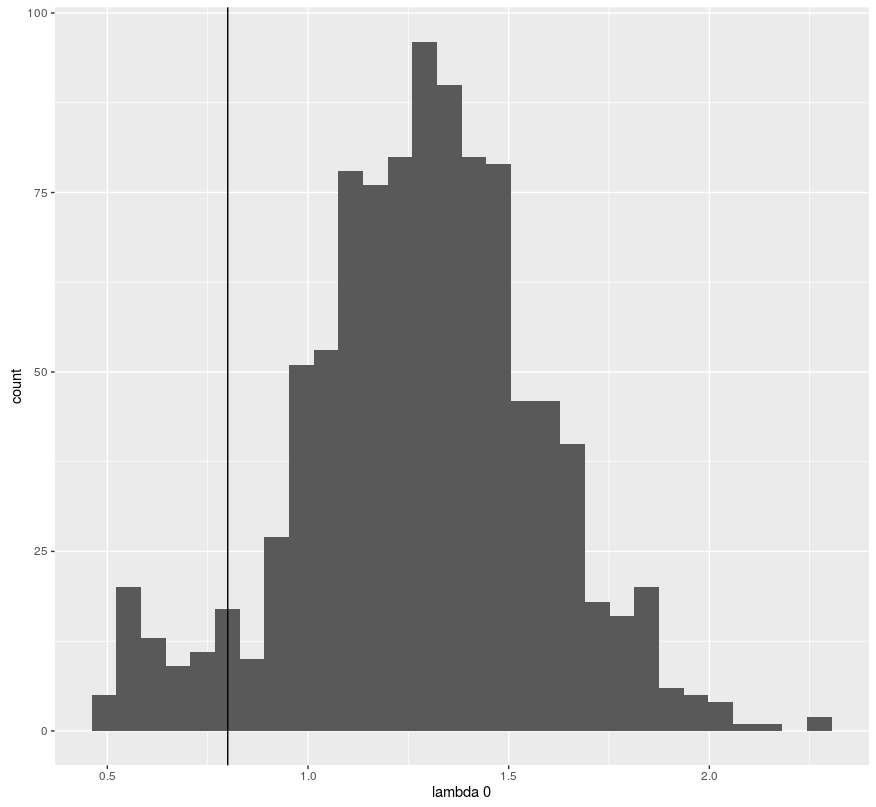
\includegraphics[width=.5\textwidth]{lambdah.png}
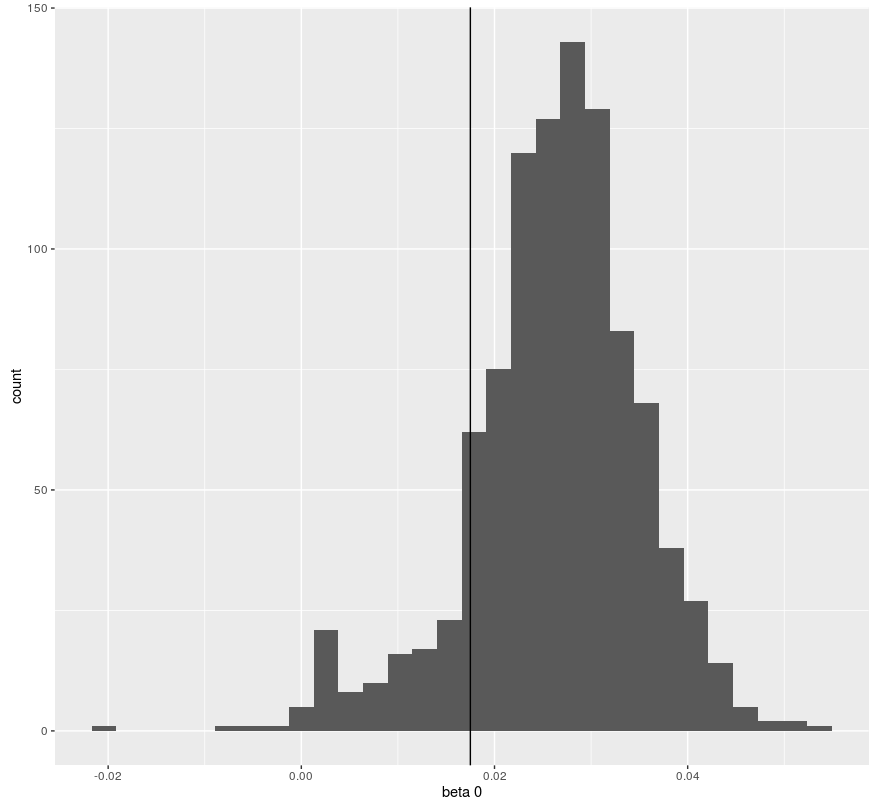
\includegraphics[width=.5\textwidth]{beta0h.png}
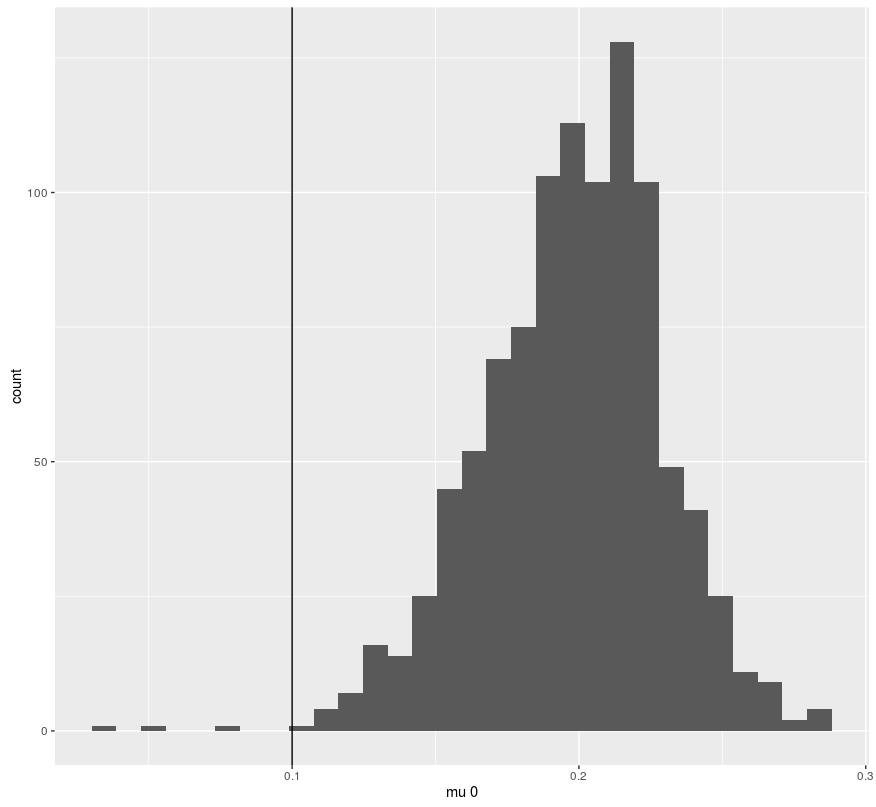
\includegraphics[width=.5\textwidth]{muh.png}
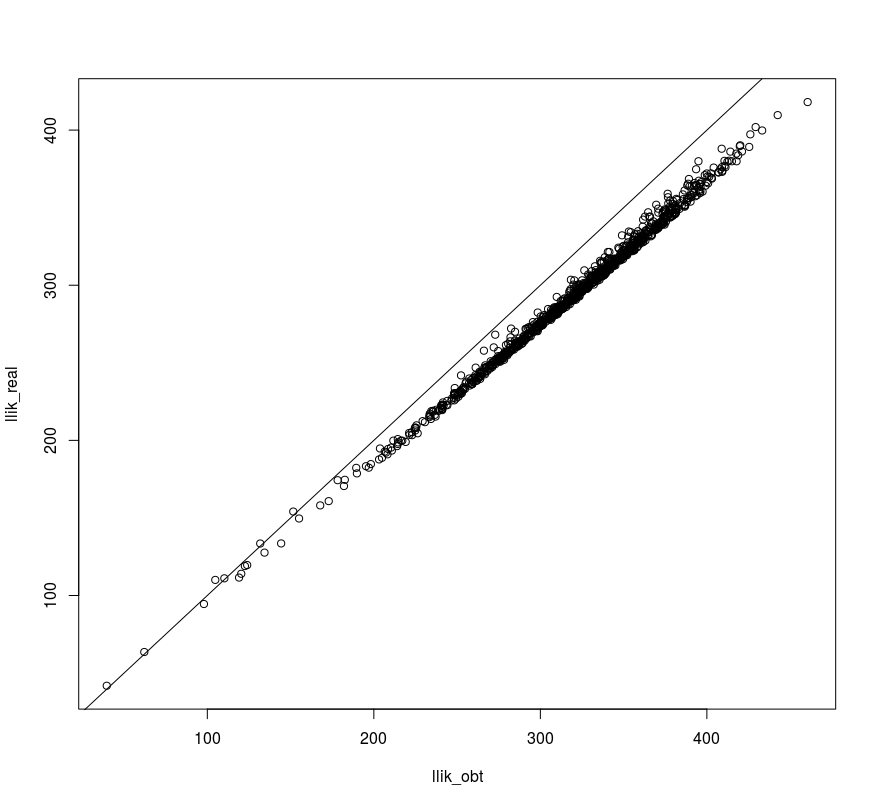
\includegraphics[width=.5\textwidth]{llikh.png}
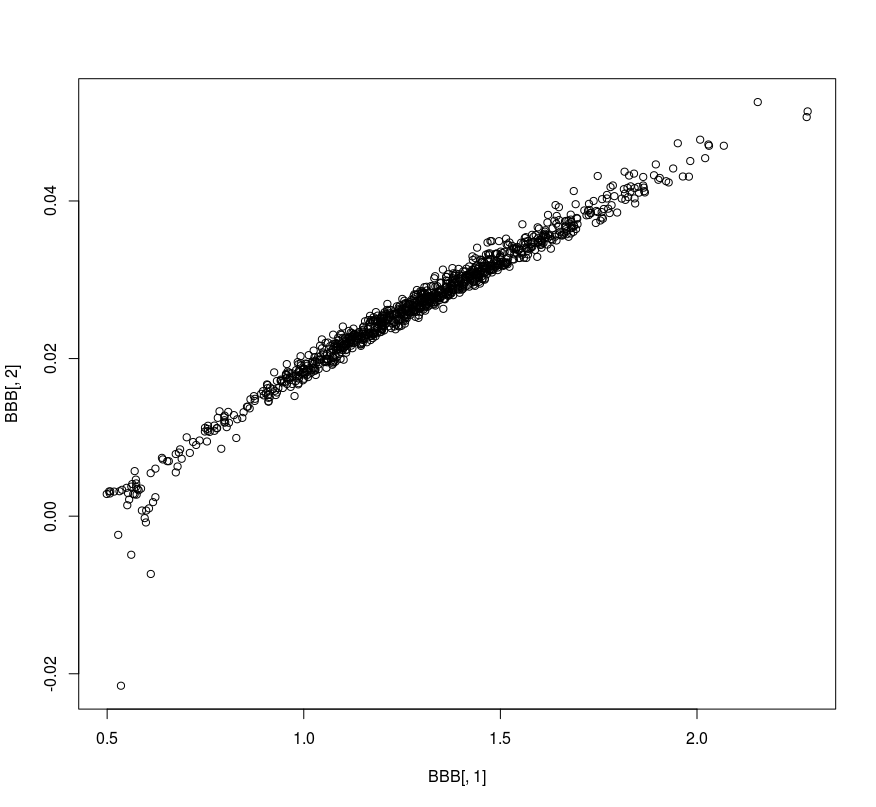
\includegraphics[width=.5\textwidth]{bolh.png}
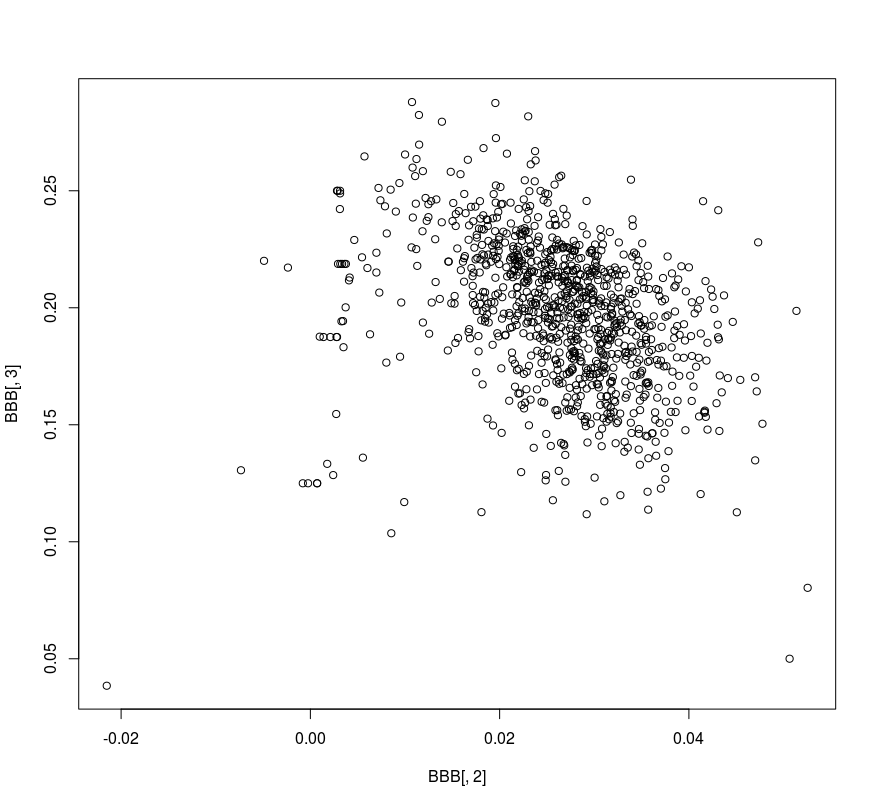
\includegraphics[width=.5\textwidth]{b0mh.png}

\end{figure}



\end{document}
